
\documentclass[main]{subfiles}
\usepackage[sols]{workbook}
\numbering{ws1-8}

\begin{document}

\ifSubfilesClassLoaded{%
  \chaptermark{\chapterone}
}{}

\section{Numerical Integration and Error Bounding} \label{ws1-8}
\begin{framed}
\textbf{Lesson Goals:}
\begin{itemize}[parsep=0pt]
\item You should be able to use the error bound formulas for $L_n$ and $R_n$ to find the maximum possible error when using a left or right-hand Riemann sum to approximate an integral. 
\item You should also be able to use the error bound formulas to find a number of slices that will ensure a certain margin of error from a Riemann sum approximation.
\item You should be able to understand and explain the error bound formulas for $T_n$ and $M_n$ including what they say, the notation they use, and the motivation behind the formulas.
\item You should be able to use the error bound formulas for $T_n$ and $M_n$ to find the maximum possible error when using these methods to approximate an integral. You should also be able to use the error bound formulas to find a number of slices that will ensure a certain margin of error from a Riemann sum approximation.
\end{itemize}
\end{framed}


\begin{framed}
\textbf{ \centerline{Error Bounds in Numerical Approximations}}
Let $ \displaystyle{I = \int_a^b  f(t)\,dt}$ and assume $f$ has a continuous derivative. Then the errors in using left and right hand sums can be bounded as follows:

\begin{multicols}{2}

\begin{center}
$|L_n - I | \leq \displaystyle \frac{  M_{(1)} (b-a)^2}{2n}$      
  
  
$|R_n - I|  \leq \displaystyle \frac{  M_{(1)} (b-a)^2}{2n}$
\end{center}


\end{multicols}
where $M_{(1)}$ is an upper bound for  $|f'|$ on $[a,b]$.

\end{framed}

\begin{enumerate}

\item\begin{problem}[\vfill]
    Look at this \href{https://www.desmos.com/calculator/0avvclvfj7}{Desmos file}. What factors make the error larger? What factors make the error smaller?
\end{problem} 

\begin{solution}
    Using more slices will decrease the error. A steeper change in slope will increase the error. A longer interval will increase the error.
\end{solution}
\item 
  \begin{problem}
Let's make sense of the formula above.
  \end{problem}
  \begin{enumerate}
   
   \item
   \begin{problem}[\vfill]
   Why does it make sense that the error bound for $L_{n}$ and $R_{n}$ depend on the derivative of $f$?
   \end{problem}

   \begin{solution}
   For each slice in the left or right-hand sum, you pretend that the function has a constant height.  It makes sense that if the function is actually changing, then there will be some error on each slice.  The faster the function is changing, the bigger we expect the error to be.
   \end{solution}

   \item
   \begin{problem}[\vfill]
   Why does the $n$ in the denominator make sense?
   \end{problem}

   \begin{solution}
   Using more and more slices makes the bound on the error smaller and smaller.  This makes sense since the narrower each slice is, the more reasonable it is to assume that the function is constant on that slice.
   \end{solution}
   
   \item
   \begin{problem}[\vfill]
   Can you make sense of the $(b-a)$ in the numerator?
   \end{problem}

   \begin{solution}
   If you're using a fixed number of slices, then as the width of the interval $(b-a)$ grows, your slices will become wider and wider.  As we know, the wider a slice is, the more potential there is for the function to change over that slice.  So we expect the error to grow as the length of the interval $(b-a)$ grows.
   \end{solution}
\end{enumerate}
\pspace{\newpage}
\item  \label{overflow-protocols}
\begin{problem}
From 1:00pm until 7:00pm water is entering a reservoir at a rate given by $f(t) = 100\sqrt{\ln t}$ gallons per 
hour, where $t$ is the number of hours after noon.  To find the amount of water that leaked into the reservoir 
between 4pm and 6pm, we must evaluate $I = \int_{4}^{6} 100 \sqrt{\ln t} \,dt$. (Why?)

This is not easy to integrate.  Edith uses $L_{5}$ to approximate the integral.  They get $L_{5}=249.744$ and concludes that about $249.744$ gallons of water entered the reservoir between 4pm and 6pm.  Overflow protocols must be put into effect if the amount of water is over $255$ gallons, so we naturally are interested in Edith's computation.
\end{problem}

\begin{enumerate}

  \item 
  \begin{problem}[.5in]
  Why is it probably futile to ask Edith for the \textit{exact} value of 
  $I = 100\int_{4}^{6} \sqrt{\ln t}\,dt$?
  \end{problem}

  \begin{solution}
  The function defined by $f(t) = \sqrt{\ln t}$ for $t \geq 1$ actually does not have an antiderivative
  that can be expressed in terms of elementary functions (polynomials, root functions, trigonometric functions,
  exponential functions, etc).  We say ``$\sqrt{\ln t}$ has no elementary anti-derivative''
  \end{solution}

  \item 
  \begin{problem}[.5in]
  Why is it probably not a good idea to ask Edith for the exact error in their computation?  That is, why 
  shouldn't you ask them for the exact value of $I-L_{5}$, the difference between the exact value of the integral
  and their approximation?
  \end{problem}

  \begin{solution}
  The only way to know the exact error is to find the difference between the approximation and the exact value of 
  $I$! Since we have no way to find the exact value of $I$, we couldn't possibly know the exact error.  Another 
  way to think of this is: if you know your approximate value, and you know the exact error, then the sum of 
  these is the exact value!
  \end{solution}

  \item 
  \begin{problem}[1.8in]
  Using the error bound for the error (given above) for $L_{5}$, give a range of possible exact values of $I = 100 \int_{4}^{6} \sqrt{\ln t}\,dt$.  Draw this range on a number line.  Your range can be ``too big'', but it's important NOT to give a range that does not include the actual value of the integral.\footnote{It turns out that $R_{5}=256.191$. It would be interesting to repeat this part using $R_{5}$ in place of $L_{5}$.  What do you think must be true about the ranges that you get in each case?} Do we have to implement the overflow protocols?
  \end{problem}

  \begin{solution}
  To begin to use the error bounding formula, we need to have a value of $M_{(1)}$, namely an upper bound for 
  $|f'(x)|$ for $x$ in $[a,b]$.  To begin, we compute the derivative by the chain-rule:

  $$\frac{d}{dt} 100\sqrt{\ln t} = \frac{100}{2}\frac{1}{\sqrt{\ln t}}\frac{1}{t} = \frac{100}{2 t \sqrt{\ln t}}$$

  We want to find a number $M_{(1)}$ that is definitely bigger than this $\frac{100}{2}\frac{1}{\sqrt{\ln 
  t}}\frac{1}{t}$ for all values of $t$ in $[4,6]$.  Because all the factors in the denominator get bigger as $t$ 
  increases, the biggest value of $\frac{100}{2 t \sqrt{\ln t}}$ is going to be when $t=4$.  So for all $t$ in 
  $[4,6]$ we have:

  $$\frac{d}{dt} \sqrt{\ln t} = \frac{1}{2 t \sqrt{\ln t}} \leq   \frac{100}{8 \sqrt{\ln 4}} \le \frac{100}{8} = \frac{25}{2}$$

  (If we have a calculator handy, we can just compute $\frac{100}{8\sqrt{\ln{4}}} \approx 10.6$.  Notice that this 
  is smaller than our upper bound, so in some sense it's a ``better'' upper bound.  But you'd really need a 
  calculator to compute it, so it's not super practical. It's useful to be able to bound functions without using a 
  calculator.  In the work above, we notice that since $e<4$, we know that $1<\ln 4$, and hence $1<\sqrt{\ln 4}$, 
  so the complicated factor in the denominator only makes the fraction smaller.)

  We get an upper bound for  the error in the $5$-slice approximation that says:

  $$|L_{5} - I | \leq \frac{  M_{(1)} (b-a)^2}{2n}  = \frac{ \frac{25}{2} (4-2)^{2}}{2(5)} = \frac{25}{5} = 5$$

  This means that the actual value of $I$ is within $5$ of the approximate value of $249.744$.  Hence the exact 
  amount of water (in hundreds of gallons) lies somewhere within the range drawn below.

  \begin{center}
  
\includegraphics[width=3in]{ws/images/reservoir-error-line-2}
  \end{center}		

  Notice that the approximate value $L_5 = 249.744$ along with this practical bound for the error is enough to 
  tell us that we don't need to use the overflow protocols.  We don't know how big the error in our approximation 
  is exactly, but we know for sure that it's less than $5$ gallons, and from the number line picture, it clearly 
  precludes the possibility that the volume of water is $255$ gallons.
  \end{solution}

  \item \begin{problem}[2in]
  Suppose that we want to approximate $I = \int_{4}^{6} 100 \sqrt{\ln t}\,dt$ with error less than $0.1$.  Using the 
  bound for the error (given above) find a value of $n$ for which you can be sure that $L_{n}$ is within $0.1$ of 
  $I$.  (Is $n$ unique?)  
  \end{problem}
 

  \begin{solution}
  We know that the actual size of the error, $|L_{n}-I|$, is certainly less than the error bound $\frac{ M_{(1)} 
  (b-a)^2}{2n}$. If we ``set the error bound less than 0.1'', we can figure out a value of $n$ that will make this 
  error bound small enough to guarantee the error is less than $0.1$.  We are free to use the same value of 
  $\frac{25}{2}$ for $M_{(1)}$, since that's still a good bound for the derivative.

  Setting $\frac{  M_{(1)} (b-a)^2}{2n} < 0.1 = 1/10$, and rearranging, we get 
  
  \begin{eqnarray*}
  \frac{ \frac{25}{2} (6-4)^2}{2n} &<& \frac{1}{10} \\
  \frac{25}{n} &<& \frac{1}{10} \\
  250 &<& n
  \end{eqnarray*}

  So, as long as we take at least 250 slices, we can be sure that our bound for the error is less than $0.1$. 
  Since the bound for the error is just that -- bigger than the error! -- we know that the error will be actual 
  error will be even smaller than that.

  \fbox{NOTE:} If, after rearranging, you end up with an equality that says $n \leq \ldots$, you should stop and 
  ask: what happened?  Does it makes sense to get an answer that was ``$n$ should be smaller than 267'', since 
  that would mean that you're not allowed to use too many slices -- but we know that the errors get EVEN SMALLER 
  when you take more slices.

  \end{solution}
\end{enumerate}
\pspace{\newpage}
\begin{framed}
\textbf {\underline{Error in Numerical Approximations:} }
Let $\displaystyle I = \int_a^b f(t)\,dt$, and assume that $f$ has a continuous second derivative.  
Then the errors in using the trapezoidal rule and the midpoint (tangent) rule satisfy the bounds
$$
  |T_n - I|  \leq  \frac{  M_{(2)} (b-a)^3}{12n^2}  \qquad \mbox{and} \qquad
  |M_n - I|  \leq  \frac{  M_{(2)} (b-a)^3}{24n^2}
$$
where $M_{(2)}$ is an upper bound for  $|f''|$ on $[a,b]$.
\end{framed}

\note{Why does it make sense that the error bounds here depend on the second derivative?  What happens when you use 
$T_n$ and $M_n$ to find the area under a line?}

%%%%%%%%%%%%%%%%%%%%%%%%%%%%%%%%%%%%%%%%%%%%%%%%%%%%%%%%%%%%%%%%%%%%% 


\item  \label{Fresnel}

\note{I'll definitely have students work on this one during class, after which we'll check in
as a class to give a thorough overview of the strategy.  This problem gets at the core of why numerical
integration is sometimes necessary, forces students to practice bounding functions, and highlights
that error bounds can help us guarantee a desired error tolerance even when the luxury of an
exact answer is impossible.}

\begin{problem}[1in]
  Fresnel integrals arise in the study of optics, and $\displaystyle I = \int_{0}^{2} \cos(x^2)~dx$ is an
  example of such an integral.  Unfortunately, the function $f(x) = \cos(x^2)$ does not have
  an antiderivative expressable in terms of elementary functions, so one must resort to approximating
  the integral.  Using the above error bounds, find a choice of $n$ which guarantees that the
  trapezoidal rule approximation $T_{n}$ is within $10^{-8}$ of the exact value of $I$.  You
  do not need to give the best (i.e., minimal) choice of $n$ that works.
\end{problem}


\begin{solution}
  Let $f(x) = \cos(x^2)$.  In order to apply the error bound for the trapezoidal rule, we need an
  upper bound $M_{(2)}$ on for $|f''(x)|$ over the domain $0 \leq x \leq 2$.

  Differentiating $f$ twice, we have $f'(x) = -2x \sin(x^2)$ and
  $$
    f''(x) = -2 \sin(x^2) - 4x^2 \cos(x^2).
  $$
  Now we estimate
  $$
    \begin{aligned}
    |f''(x)| & = |-2 \sin(x^2) - 4x^2 \cos(x^2)|  \\
             &  \leq |-2 \sin(x^2)| + |-4x^2 \cos(x^2)|  \qquad \mbox{(by the triangle inequality)} \\
             & = |2| |\sin(x^2)| + |4x^2| |\cos(x^2)| \\
             & \leq 2 + 4x^2 \qquad \mbox{(by boundedness for sine and cosine functions between -1 and 1)}.
    \end{aligned}
  $$
  Thus, on the domain $0 \leq x \leq 2$, we have $|f''(x)| \leq 18$.  Using the error bound
  for the trapezoidal rule with $M_{(2)} = 18$ and $a = 0$ and $b = 2$, we are guaranteed that
  $$ 
    |T_{n} - I| \leq \frac{18(2-0)^3}{12 n^2} \; = \; \frac{12}{n^2}.
  $$
  We \textbf{want} to ensure that $|T_{n} - I| \leq 10^{-8}$ and we {\bf know} that
  $|T_{n} - I| \leq 12/n^2$.  Thus, if we insist that $12/n^2 \leq 10^{-8}$, then we'll
  have the assurance that the error is within the desired tolerance.  By algebra,
  $$
    \frac{12}{n^2} \leq \frac{1}{10^{8}}
  $$
  is equivalent to
  $$
    n^2 \geq 12 \times 10^8.
  $$
  To facilitate computation of square roots by hand, let's just insist that
  $$
    n^2 \geq 16 \times 10^8,
  $$
  from which it follows that $n \geq 4 \times 10^4$.  In other words, using $n = 40000$
  guarantees that $T_{n}$ is accurate to within the desired tolerance.
  \end{solution}
\pspace{\newpage}
  \item In this problem you will consider numerical approximations to the integral $I = \int_1^5 \arctan \sqrt{x}~dx$. Below you can find the graph of the function $f(x) = \arctan \sqrt{x}$ as well as its first and second derivatives.

\begin{minipage}{0.5\textwidth}
\begin{center}
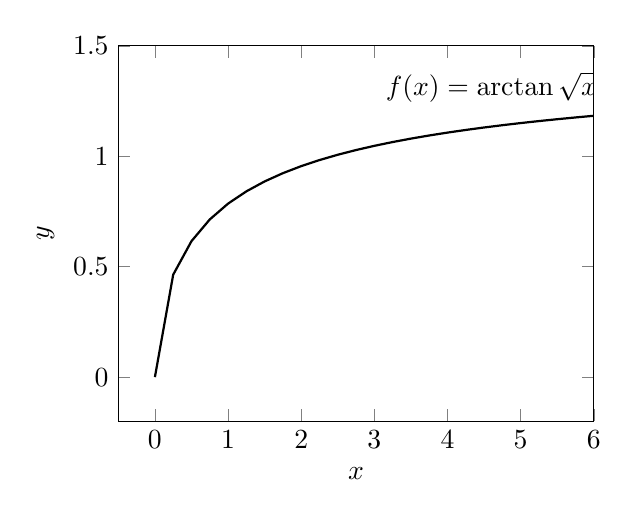
\begin{tikzpicture}
    \begin{axis}[%axis lines = left, 
        xlabel = $x$, ylabel = $y$,
        width=3in,
        height=2.5in,
        xtick={-1,0,...,7},
        ytick={-0.5,0,...,3},
        xmin=-0.5,
        xmax=6,
        ymin=-0.2,
        ymax=1.5]
        \addplot[domain=0:6,style= thick]{rad(atan(x^0.5))};
        \node [above] at (4.6,1.2) {$f(x)=\displaystyle\arctan \sqrt{x}$};
   \end{axis}
\end{tikzpicture}  
\end{center}
\end{minipage}
\begin{minipage}{0.5\textwidth}
    \begin{center}
        $$f(x) = \arctan (\sqrt{x})$$

        \vspace{-0.1in}
        
        $$f'(x) = \frac{1}{2\sqrt{x}(1+x)}$$

        $$\displaystyle f''(x) = -\frac{3x+1}{4x^{\frac32}(1+x)^2}$$
    \end{center}
\end{minipage}

\begin{enumerate}
\item Determine whether each statement below is True or False and justify your choice. Each solution should include a separate picture as part of your explanation. We use $L_n$, $R_n$, $T_n$ and $M_n$ to represent the left-hand, right-hand, trapezoidal and midpoint rules, respectively.

\begin{enumerate}
    \item 
    \begin{problem}[1.5in]
    $M_4$ is an overestimate for the integral $I$.  \qquad \framebox(10,10){\solonly{\textcolor{blue}{\checkmark}}} \textbf{ True} \hspace{0.2in} \framebox(10,10){} \textbf{ False}
    \end{problem}

    \begin{solution}
        We can conclude the statement is \textbf{True} based on a single-slice analysis, interpreting $M_4$ as a midpoint tangent sum. On the picture below we see the trapezoid given by the midpoint tangent line has bigger area than then the area under the function.

\begin{center}
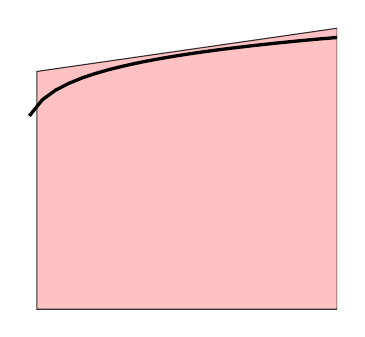
\begin{tikzpicture}
    \begin{axis}[axis lines = none, 
        xlabel = $x$, ylabel = $y$,
        width=2.5in,
        height=4in,
        xtick={-2,-1,...,3},
        ytick= {0,0.5,1,...,2},
        ticks = none,
        xmin=0.5,
        xmax=3,
        ymin=0,
        ymax=2.5]
        \filldraw[fill=red!30, opacity=0.8](1,0) -- (1,0.88) -- (3,1.04) -- (3,0)-- cycle;
        \addplot[domain=0.95:3.05,style= very thick]{(0.5*(x-0.88))^0.1};
    \end{axis}
\end{tikzpicture}
\end{center}

    \end{solution}

    
    \item
    \begin{problem}[1.5in]
    $M_2 < T_2$. \qquad \framebox(10,10){} \textbf{ True} \hspace{0.2in} \framebox(10,10){\solonly{\textcolor{blue}{\checkmark}}} \textbf{ False}
    \end{problem}

    \begin{solution}
    Looking at a single slice below we can notice that the green trapezoid, following the trapezoidal rule has smaller area than the midpoint tangent trapezoid, so the satement is \textbf{False}.
        \begin{center}
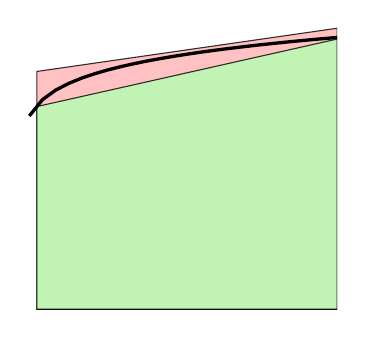
\begin{tikzpicture}
    \begin{axis}[axis lines = none, 
        xlabel = $x$, ylabel = $y$,
        width=2.5in,
        height=4in,
        xtick={-2,-1,...,3},
        ytick= {0,0.5,1,...,2},
        ticks = none,
        xmin=0.5,
        xmax=3,
        ymin=0,
        ymax=2.5]
        \filldraw[fill=red!30, opacity=0.8](1,0) -- (1,0.88) -- (3,1.04) -- (3,0)-- cycle;
        \filldraw[fill=green!30, opacity=0.8](1,0) -- (1,0.75) -- (3,1) -- (3,0)-- cycle;
        \addplot[domain=0.95:3.05,style= very thick]{(0.5*(x-0.88))^0.1};
    \end{axis}
\end{tikzpicture}
\end{center}
    \end{solution}

    \item
    \begin{problem}[1.5in]
    $|R_2-I| < |L_2-I|$. \qquad \framebox(10,10){\solonly{\textcolor{blue}{\checkmark}}} \textbf{ True} \hspace{0.2in} \framebox(10,10){} \textbf{ False}
    \end{problem}

    \begin{solution}
   We see below that the error associated to the right hand sum (represented in yellow) is smaller than the error associated to the left hand sum (represented in blue), so the statement is \textbf{True}.

    \,

    \,
    \vspace{-2in}
     
        \begin{center}
\begin{tikzpicture}
    \begin{axis}[axis lines = none, 
        xlabel = $x$, ylabel = $y$,
        width=2.5in,
        height=4in,
        xtick={-2,-1,...,3},
        ytick= {0,0.5,1,...,2},
        ticks = none,
        xmin=0.5,
        xmax=3,
        ymin=0,
        ymax=2.5]
        \addplot[domain=1:3, name path = A]{1};
        \addplot[domain=1:3, name path = B]{0.75};
        \addplot[domain=0.95:3.05,style= very thick, name path = C]{(0.5*(x-0.88))^0.1};
        \draw(1,0) -- (1,1) -- (3,1) -- (3,0)-- cycle;
        \addplot[yellow!40, opacity=0.6] fill between [of=A and C,soft clip={domain=1:3}];
        \addplot[blue!40, opacity=0.6] fill between[of=C and B,soft clip={domain=1:3}];
    \end{axis}
\end{tikzpicture}
\end{center}
    \end{solution}
    
\end{enumerate}
\pspace{\newpage}
    \item
    \begin{problem}[2in]
    Find a practical value for $M_{(2)}$.
    \end{problem}

    \begin{solution}
        $M_{(2)}$ is an upper bound for $|f''(x)|$. Notice that on the interval $[1,5]$ we have:

        \[|f''(x)| = \frac{|3x+1|}{4|x^{3/2}||1+x|^2} \leq \frac{16}{4 \cdot 2^2} = 1\]

        Above we used the choice $x = 5$ in the numerator and $x=1$ in the denominator to get a safe upper bound for the fraction. Thus we can set \fbox{$M_{(2)} = 1$}.

    \end{solution}

    \item 
    \begin{problem}[3in]
    Suppose you want to approximate $I$ using the trapezoidal rule $T_n$ and you want to make sure that the error in your approximation is less than $10^{-6}$. How many slices should you use? Remember, you do not need to give the smallest number of slices that works, just a reasonable integer (whole number) that guarantees that the error is less than $10^{-6}$. Explain your reasoning.
    \end{problem}

\begin{solution}
To guarantee that the error is smaller than $10^{-6}$ it is enough to find $n$ such that 
\[\frac{M_{(2)}(b-a)^3}{12n^2} \leq 10^{-6}\]

Using $M_{(2)} = 1$ from above, $a = 1$, $b=5$ we get
\[\frac{4^3}{12n^2} \leq \frac{1}{10^{6}}\]
That is,
\[n^2 \geq \frac{16}{3} \cdot 10^6\]
or yet
\[n \geq \frac{4}{\sqrt{3}} \cdot 10^3\]
Since $\frac{1}{\sqrt{3}} \leq 1$ it is enough to pick \fbox{$n = 4000$}

\end{solution}

\end{enumerate}



 \end{enumerate}

 \end{document}